%!TEX root = ./main.tex
%!TEX encoding = UTF-8 Unicode
\chapter{Description of instructions binary code}
\label{chap:format}
The description of the instruction format is based on a tree structure, allowing up to pool the common format of each instruction. The objective here is to extract from the binary format of instruction, both the type of instruction, and the operands. In the generated simulator, this step takes place in the \emph{decoding} phase of instructions.

We will study in a first approach fixed size instruction set. The description will then be extended to variable size instruction sets in section \ref{sec:formatTailleVariable}.

\section{General architecture}
The description of the binary format will allow to decode the binary format of instructions. Initially, it is necessary to provide in section \texttt{default} the basic size of instructions:
\begin{lstlisting}
default {
    instruction := 16  -- default instruction size in bits
}

\end{lstlisting}
In this example for instance, the instruction size is 2 bytes or a multiple of 2 bytes for the variable-size instruction sets. For example, instructions sizes in the \texttt{HCS12} are from 1 to 8 bytes. In this case, you should specify \texttt{instruction := 8}.

The description of the format describes how to decode the binary word whose size is supplied.

The general structure of the description of format nodes is:
\begin{lstlisting}
format <name> [tag]
  <formatBody>
end format
\end{lstlisting}

\texttt{<formatBody>} is a sequence of elements:
\begin{itemize}
\item \emph{tags};
\item call to another format
\item select structure, using the \texttt{select} keyword. See section \ref{sec:formatSelect};
\item definition of operands. See section \ref{sec:operandeFormat}.
\end{itemize}

\subsection{Select structure}
\label{sec:formatSelect}
The \texttt{select} statement allow to differentiate different branches of the tree, like in the description of each view.

The select statement acts on a bit field of the binary format of the instruction:
\begin{lstlisting}
  select slice <field>
    case <masque> is <formatBody>
    case .. 
  end select
\end{lstlisting}

\subsubsection{\texttt{field} part}
The \texttt{field} part indicate the binary part of the instruction code that will be used to differentiate instructions. For example, let's consider instructions \texttt{ADDC} and \texttt{ADD} of AVR, where the binary representation is given in figure \ref{fig:selectFormat1}.

\begin{figure}[h]		%% select sur ADD et ADDC
  \begin{center}
    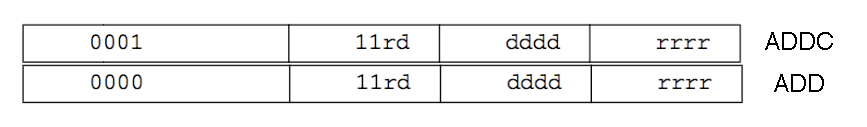
\includegraphics[width=0.8 \linewidth]{../common/images/selectFormat1.pdf}
    \caption{Binary code of instructions \texttt{ADDC} and \texttt{ADD} of Atmel AVR® (code size is 16 bits).}
    \label{fig:selectFormat1}
  \end{center}
\end{figure}

In this case,the following construction can be used:
\begin{lstlisting}
  select slice {12}
    case 0 is ... -- ADC
    case 1 is ... -- ADD
  end select
\end{lstlisting}

Indeed, only bit 12 distinguishes the 2 instructions. The \texttt{<field>} part is written in the same way than a bitfield of a variable (section \ref{sec:field}), but only numerical values can be used (no expressions):
\begin{lstlisting}
  select slice {12..10, 3..2} -- select bits 12 to 10 and 3 to 2 (5 bits selected)
\end{lstlisting}
The  \texttt{<field>} part size should be guessed statically.

\subsubsection{\texttt{mask} part}
The \texttt{mask} part operates on bit fields taken from the \texttt{field} part. It could not have a higher size than the \texttt{field} one (an error is generated during generation of the simulator).

The \texttt{mask} part can be either a numerical value (as in the previous example) or a binary mask (see section \ref{masque}). When using a binary mask, charater \texttt{-} can either be understood as a \texttt{0} or \texttt{1}. Using the example of figure \ref{fig:selectFormat1}, if we want to pool the common part of the 2 instructions:
\begin{lstlisting}
  select slice {15..10}
    case \m000-11 is .. -- both ADD and ADDC
    case ...
  end select
\end{lstlisting}
In this case, a selection is done on the whole \emph{opcode} (binary code except the operands). The first \texttt{case} will be taken only if bits \texttt{15..10} are \texttt{000011} (\texttt{ADD}) or \texttt{000111} (\texttt{ADDC}).

The \texttt{or} operator allow to select different mask for one case:
\begin{lstlisting}
select slice {7..0}
    case \x1B or \x1A or \x19 is ...
    ..
\end{lstlisting}
This example, extracted from the description of the Freescale \emph{HCS12}, allow to pool different cases, although their correspondence at the binary level is not possible.

Eventually, all the other case may be pooled using the \texttt{others} keyword.
\begin{lstlisting}
  select slice {2..0}
    case \m110 is ...
    case \m111 is ...
    others     is ...
  end select
\end{lstlisting}
In this example, the last choice will be taken for all formats that not match \texttt{11-}.

The \texttt{others} keyword can only be used one time in a \texttt{select} statement, and it should be the last case.

\subsubsection{\texttt{<formatBody>} part}
The \texttt{<formatBody>} is the body of a \emph{format} node.

\subsection{Extracting operands}
\label{sec:operandeFormat}
The extraction of operands use the \texttt{slice} keyword, with a bitfield. Given the 2 instructions \texttt{ADD} and \texttt{ADDC} in figure \ref{fig:selectFormat1}:
\begin{lstlisting}
  r := slice{9, 4..0} -- size: 5 bits
  d := slice{8..4}    -- size: 5 bits
\end{lstlisting}
Size of operands is computed statically. In other views (\emph{behavior} and \emph{syntax}), operands values can be retrieved as constant. In that case, the \texttt{field} keyword is used:
\begin{lstlisting}
  field u5 r
  field u5 d
\end{lstlisting}

Some operands need to be declared as signed values (for a branch for example). This is done using the \texttt{signed} keyword:
\begin{lstlisting}
  k := signed slice{11..0}
\end{lstlisting}
\texttt{k} type is \texttt{s12}.

Eventually, it may be useful to operates directly on the operands. A shift operator is provided (limited to a numerical value):

\begin{lstlisting}
  RdIndex := slice{7..4} << 1
\end{lstlisting}
In that case, \texttt{RdIndex} type is \texttt{u5}.

\section{Example}

This example is based on a part of the XGate instruction set. XGate is a co-processor integrated in the \emph{HCS12X}. It is based on a RISC architecture, with a 16 bits, fixed sized, instruction set. 16 GPR (8 bits) are provided.

\subsection{Description of a part of the instruction set of XGate}
Figure \ref{fig:shiftAndTriadicInstFormat} gives the binary format of shift and triadic instructions.

\begin{figure}[h]		%% select sur ADD et ADDC
  \begin{center}
    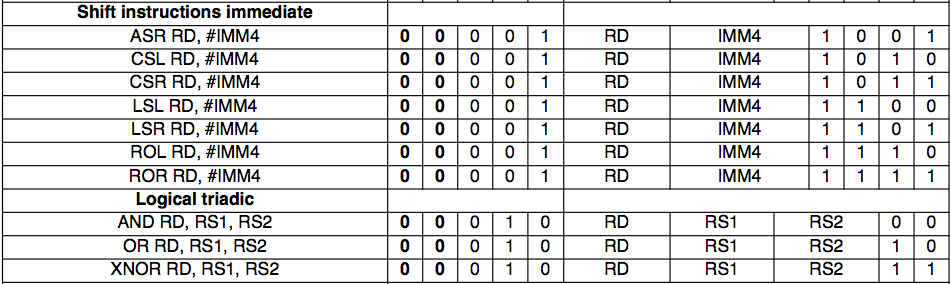
\includegraphics[width=0.95 \linewidth]{../common/images/shiftAndTriadicInstFormat.png}
    \caption{Binary code of shift and triadic instructions of XGate® \emph{Source Freescale}}
    \label{fig:shiftAndTriadicInstFormat}
  \end{center}
\end{figure}

We can directly note on this example that the bit 12 serves to differentiate the 2 types of instructions. More generally for the whole instruction set, the 5 most significant bits allow to identify instruction families (\emph{opcode}):
\begin{lstlisting}
format inst
  select slice {15..11}
    case \b00001 is shiftInstructionImm
    case \b00010 is logicalTriadic
  end select
end format
\end{lstlisting}
For shift instructions, the \texttt{shiftInstructionImm} format node is used:
\begin{lstlisting}[firstnumber=7]
format shiftInstructionImm #IMM
  rdIndex := slice{10..8}
  imm4 := slice{7..4}
  select slice {3..0}
    case \b1001 is #ASR
    case \b1010 is #CSL
    case \b1011 is #CSR
    case \b1100 is #LSL
    case \b1101 is #LSR
    case \b1110 is #ROL
    case \b1111 is #ROR
  end select
end format
\end{lstlisting}
The instructions identification is \texttt{\#IMM \#ASR} for instruction \texttt{ASR}, \texttt{\#IMM \#CSL} for \texttt{CSL}, \ldots

For triadic instructions, the format node is:
\begin{lstlisting}[firstnumber=20]
format logicalTriadic #Triadic
  rdIndex := slice{10..8}
  rs1Index := slice{7..5}
  rs2Index := slice{4..2}
  select slice {1..0}
    case \b00 is #AND
    case \b10 is #OR
    case \b11 is #XNOR
  end select
end format
\end{lstlisting}
Thus, we have described here the binary format of these 10 (simple) instructions in 29 lines.

\subsection{Decoder generation}
The decoder may be generated, even if the other views (syntax and behavior) are not written. In that case, the following options should be given:
\begin{verbatim}
$ gadl --no-behavior --no-deasm test.hadl
\end{verbatim}
This allow to detect both syntax and semantic error in the format description. 

Moreover, it detects the orthogonality of the instruction set (a binary code can be associated to only one instruction). This verification may require computation time (few seconds for 1500 instructions) and can be removed when the binary description is done using option \texttt{--no-check}.

\subsection{Output log file}

The generated decoder files are located in \texttt{instDecoder.h} and \texttt{instDecoder.cpp}. Some other files are generated for debugging phase

Files \texttt{format\_all.dot} and \texttt{format\_ref.dot} allow to display the format tree related to instructions, in GraphViz format. The first one display the whole format (including \emph{format} names \emph{select} part), see figure \ref{fig:formatAllTest}. 

\begin{figure}[h]		%% format All
  \begin{center}
    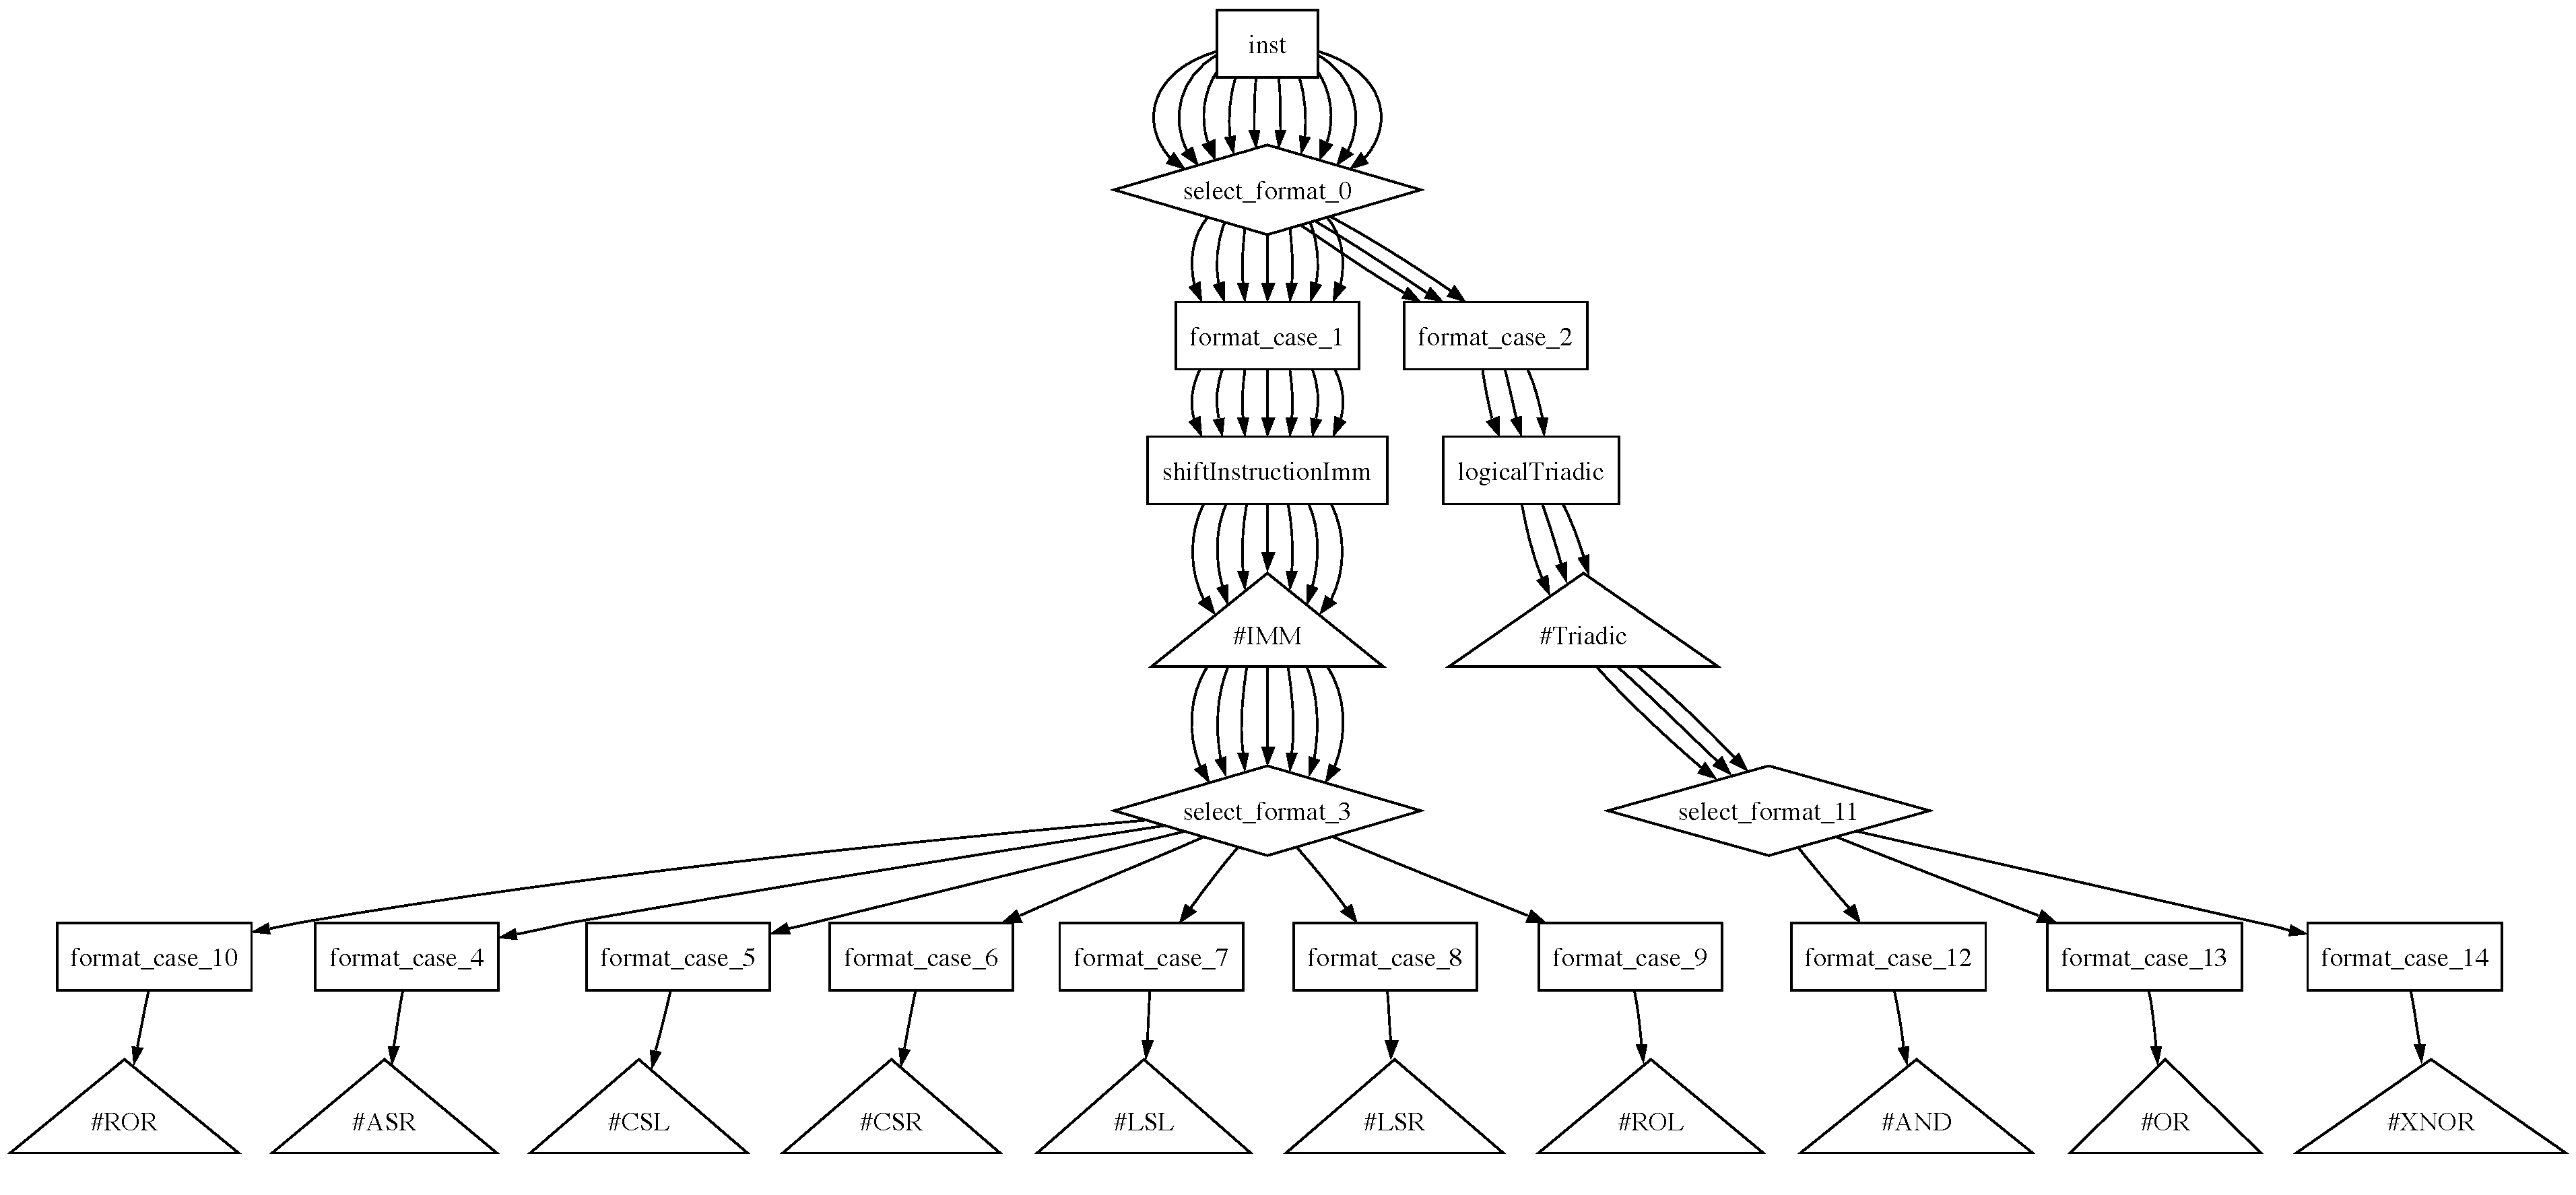
\includegraphics[width=\linewidth]{../common/images/format_all_test.pdf}
    \caption{Arbre généré à partir de la description du code binaire des instructions de décalage (shift) et les instruction triadiques (3 registres) sur la XGate.}
    \label{fig:formatAllTest}
  \end{center}
\end{figure}


This tree may become quickly difficult to display, that's why the second one only display \emph{tags} for each instruction, see figure \ref{fig:formatRefTest}. In this last figure, there are 2 distinct trees, because shift instruction and triadic instruction do not share anu common properties (no \emph{tags}).


\begin{figure}[h]		%% format Ref
  \begin{center}
    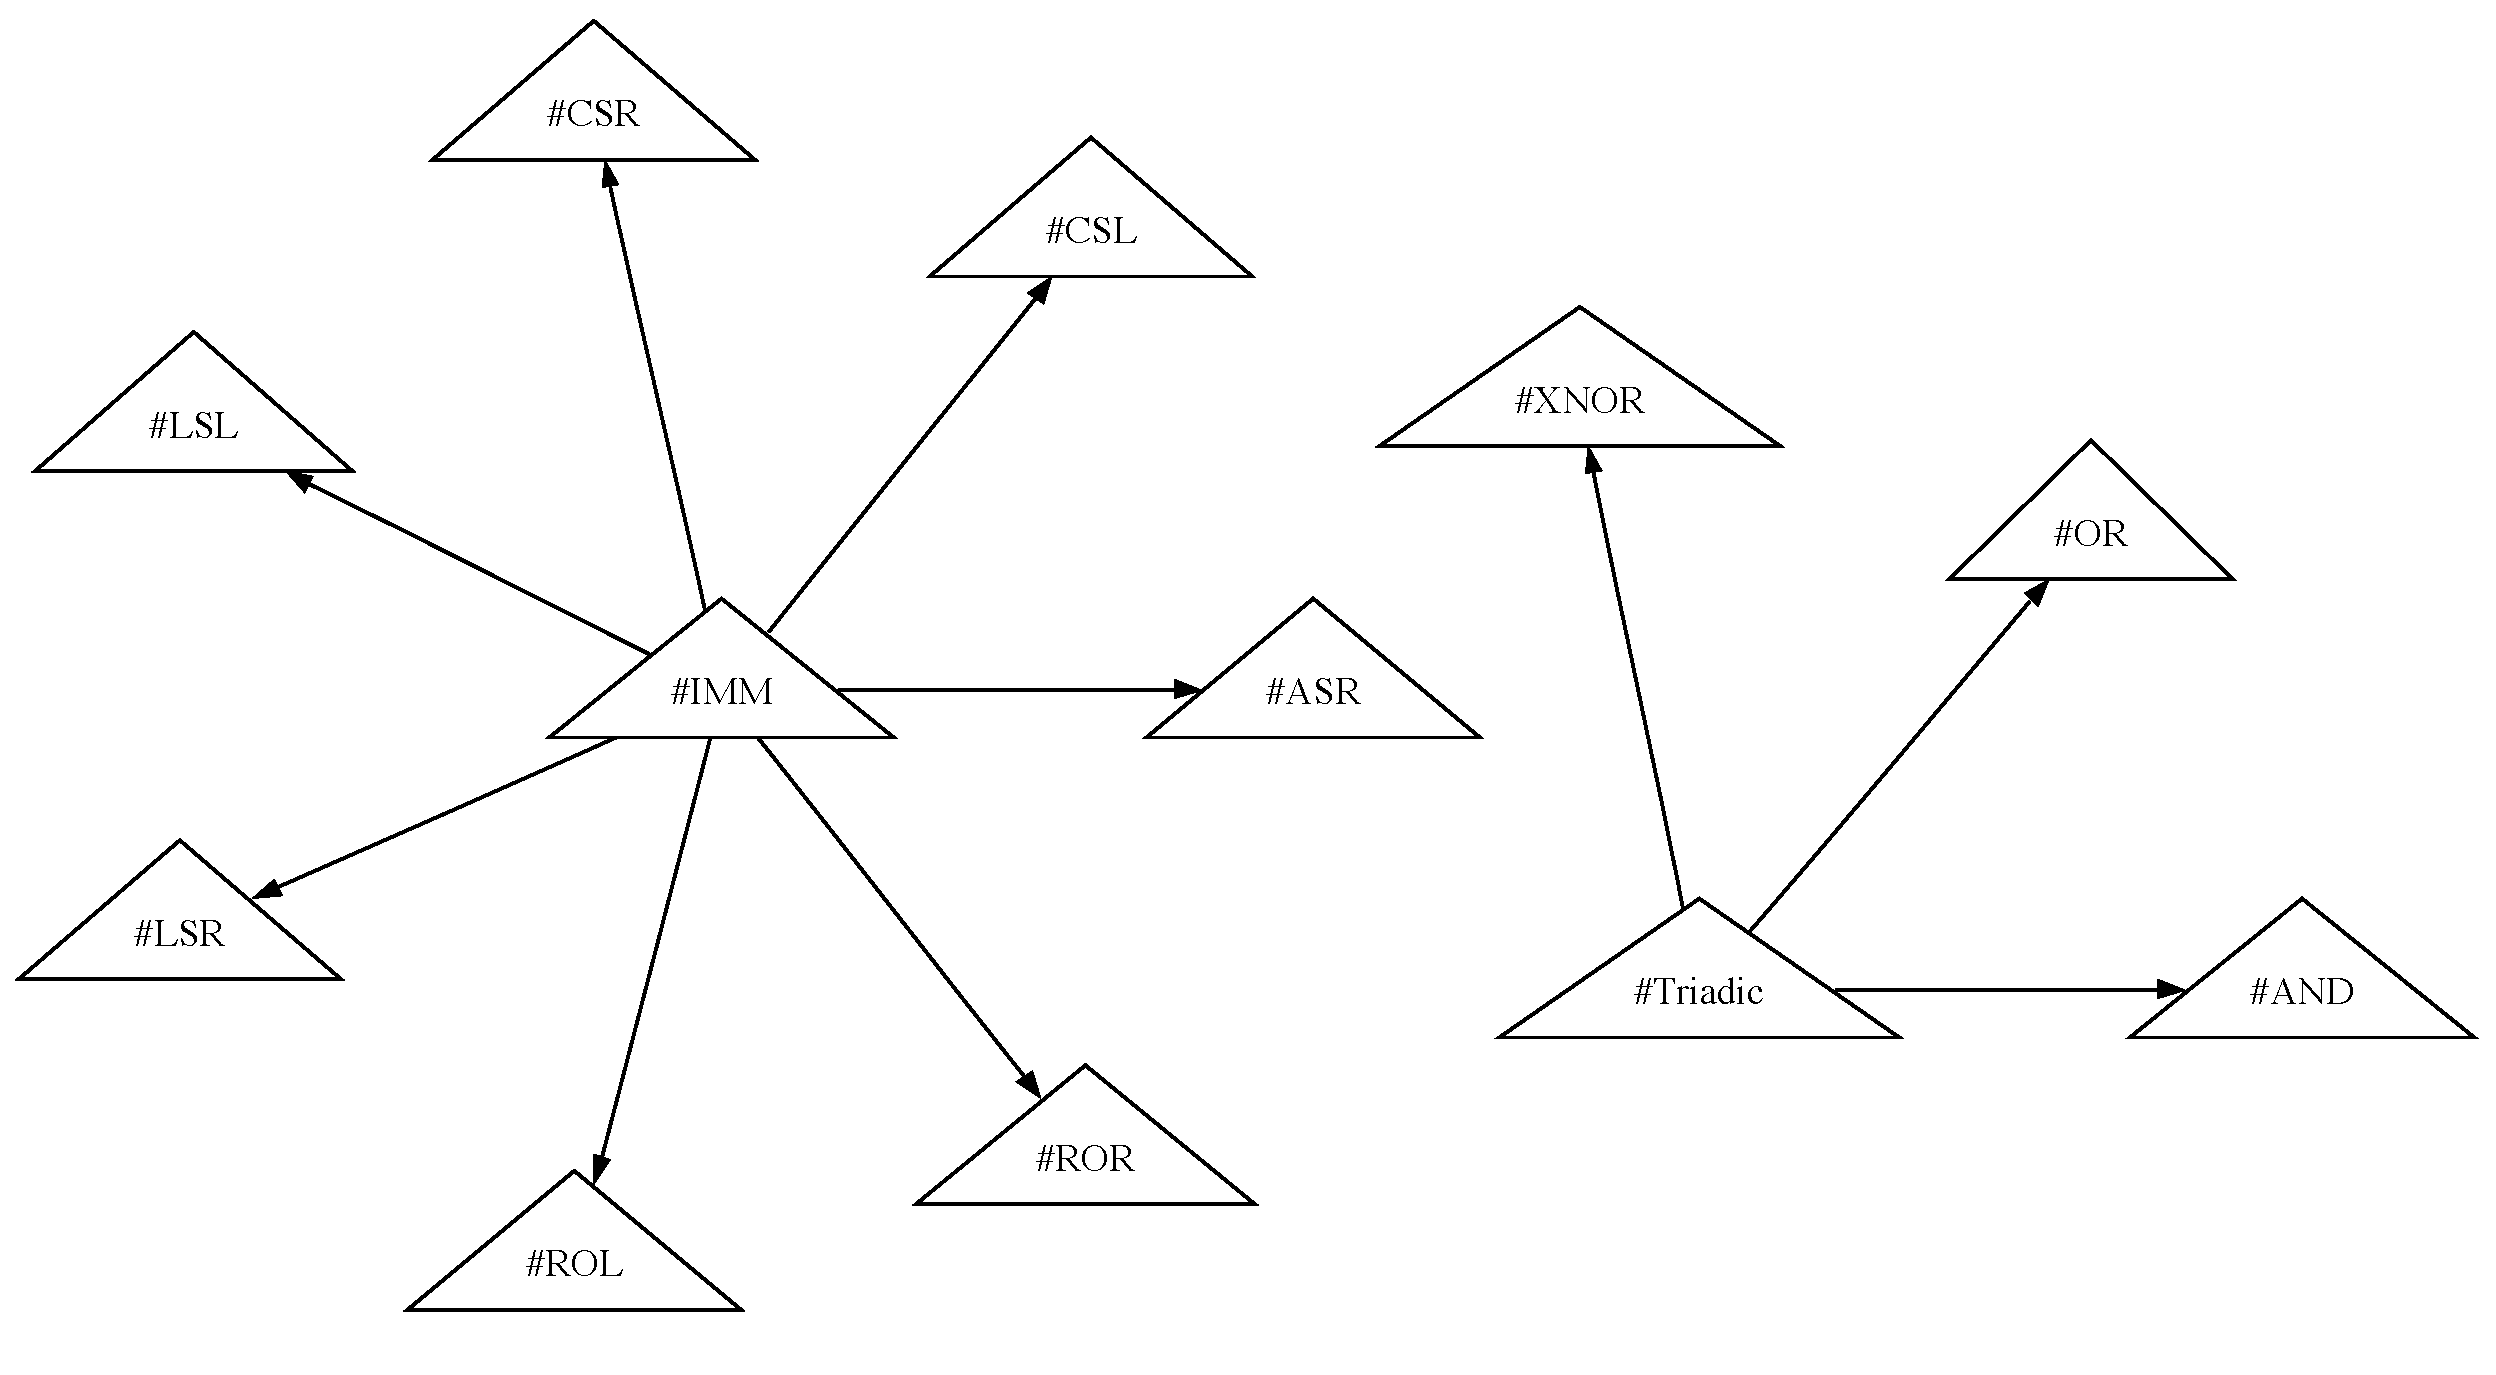
\includegraphics[width=\linewidth]{../common/images/format_ref_test.pdf}
    \caption{Trree generated from the description of shift and triadic instructions on the XGate instruction set. This tree is limited to tags.}
    \label{fig:formatRefTest}
  \end{center}
\end{figure}

Another file is \texttt{instruction.log} that embeds information about binary code of instructions:
\begin{itemize}
\item the path followed in the tree to get the instruction;
\item the \emph{instruction id}: Tags are ordered in alphabetical order;
\item the internal name used by instruction (debug in the generated \emph{C++} files)
\item the binary opcode (no date fields)
\item the name and size of data fields
\item the size of the instruction (word size is defined in section \emph{default});
\end{itemize}

For the triadic instruction \texttt{AND}, we get the following information:
\begin{verbatim}
inst 
-> select_format_0 
-> format_case_2 
-> logicalTriadic 
-> #Triadic 
-> select_format_11 
-> format_case_12 
-> #AND
	instruction id :#AND, #Triadic
	Internal name :test_AND_Triadic
	Binary coding :00010---------00
	data field(s) :rdIndex (3 bits)
	               rs1Index (3 bits)
	               rs2Index (3 bits)
	Instruction code size :1
\end{verbatim}

%TODO: debug -> fichier de log
%intérêt de l'archi avec les codes de l'ARM.
%indiquer que les performances du décodeur ne dépendent pas de la structure de l'arbre de description.

\section{variable size instruction set}
\label{sec:formatTailleVariable}
Variable size instruction set are described by adding binary words directly in the nodes.
In the following example, extracted from the \texttt{Freescale HCS12} instruction set (instruction word is 8 bits):
\begin{lstlisting}
format Instruction 
  select slice {7..0}
    case \x18 is inst_18 
    ....
  end select
end format

format inst_18 
  select slice +{7..0}
    case \m00010111 is #CBA       -- 17h
    ...
  end select
end format
\end{lstlisting}
In this example, the first node (\texttt{Instruction}) allows to defined the first word (as in fixed size instruction sets). Node \texttt{inst\_18} is called if this first word \texttt{0x18}. In format \texttt{inst\_18}, the \texttt{+} in the \texttt{select} part, line 9 implies that it is necessary to add a binary word to decode the instruction.
In this way, semantics of \texttt{+\{7..0\}} is: \emph{adding one word, and apply the \texttt{select} on the 8 bits of this new word.}

A \texttt{select} that have the following form:  \texttt{\{a..b\}\{c..d\}+\{e..f\}\{-\}\{g..h\}} show that 3 words are added for instructions de the current branch, and the \texttt{select} is applied on:
\begin{itemize}
\item bit field \texttt{a..b} of the previous word;
\item bit field \texttt{c..d} of the current word;
\item bit field\texttt{e..f} of the first word added;
\item the second added word is not used in the select structure;
\item bit field\texttt{g..h} of the third word added;
\end{itemize}
If there was no word previously added (there is only the current word), an error is generated.

If a new format is called in or after the \texttt{select}, le last added word becomes the current word.

This approach using relative access (adding words to previously added words) allow to describe easily instruction formats where the addressing mode is not always at the same place, as in the example figure \ref{fig:formatLongueurVariable}.

\begin{figure}		%% Small Example
  \begin{center}
    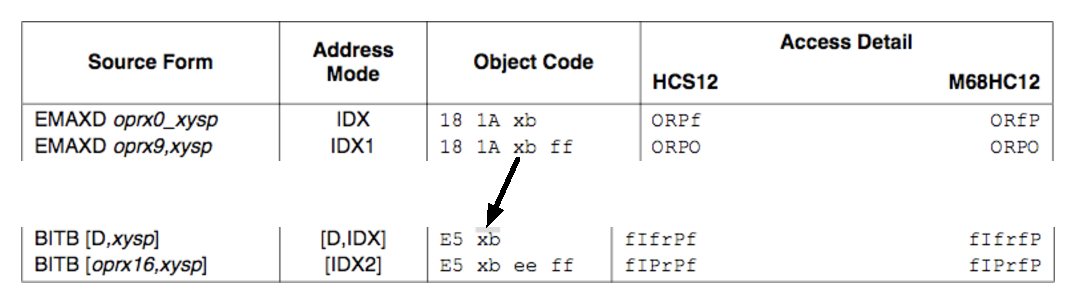
\includegraphics[width=0.8 \linewidth]{../common/images/formatLongueurVariable.pdf}
    \caption{Example of variable size instruction set, extracted form the documentation of HCS12. The addressing mode \texttt{xb} may be located at different places (source Freescale).}
    \label{fig:formatLongueurVariable}
  \end{center}
\end{figure}

%TODO: rajouter le fetch explicite!!!